\documentclass[a4paper]{article}
\usepackage[dutch]{babel}
\usepackage{geometry}
\usepackage[utf8]{inputenc}
\usepackage{hyperref}
\usepackage{listings}
\usepackage{graphicx}
\usepackage[x11names, rgb, html]{xcolor}

% dimensions
\geometry{left=3cm, top=3cm, right=3cm, bottom=3cm}

% font
\usepackage{DejaVuSans}
\renewcommand*\familydefault{\sfdefault}
\usepackage[T1]{fontenc}

% hyperlinks
\hypersetup{%
  colorlinks=true,
  linkcolor=blue,
  urlcolor=cyan,
}

% image
\graphicspath{{img/}}

% lists
\providecommand{\tightlist}{%
\setlength{\itemsep}{0pt}\setlength{\parskip}{0pt}}

% preamble
\title{Experiments}
\author{Tim Visée \& Nathan Bakhuijzen}
\date{October 2018}

\begin{document}

  \pagenumbering{gobble}
  \maketitle
  \begin{figure}[h]
    \centering
    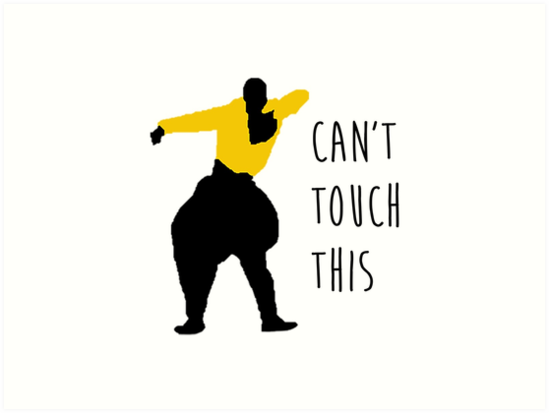
\includegraphics[width=\linewidth]{cant-touch-this}
  \end{figure}
  \clearpage

  \section{Recognized motions}
  In this document, we will list all the motions that are recognized by
  \textit{Can't Touch This}. These experiments can be conducted by first setting
  up the platform itself. Instructions for this can be found in the manual.
  After setting everything up, conducting the experiments is a piece of cake.
  Start up the platform, open a webbrowser and go to
  \href{http://localhost:8000}. Click on 'Visualize' to view your fingers being
  traced.\\

  Please try to make the following gestures above the LeapMotion sensor. You
  will receive visual feedback if a gesture has been made succesfully. Try to
  succesfully complete each gesture at least 5 times for consistency sake.

  \begin{itemize}
    \tightlist
    \item Straight line
    \item Circle clockwise
    \item Circle counter-clockwise
    \item Big circle clockwise
    \item Big circle counter-clockwise
    \item Triangle clockwise
    \item Triangle counter-clockwise
    \item Mini square clockwise
    \item Square clockwise
    \item Square counter-clockwise
  \end{itemize}

\end{document}
